\section{Results} \label{results}

For the results reported here, the CA population is 100, selection is tournament with elitism, offspring CA populations are created with both 
mutation and crossover, the IC length is 121, the size of the IC test set is 100, and CAs are run for a maximum of 
300 iterations per IC over 50 generations. When rules are referred to using decimal notation, the encoding follows Mitchell 
\cite{Mitchell:1994:ECA:186092.186116}. See section \ref{sec:methods} 
for more information regarding methods.

\subsection{Comparing neighborhoods} \label{sec:2_1}
Our first goal was to compare rules with different neighborhoods. In particular, there is a tradeoff between the size of the search space and the 
the amount of information available for purposes of setting a location state. Larger neighborhoods have rules that can 'see' more of the source IC, and 
hence (intuitively) make a more informed decision about how to set the output bit, but this comes at a cost of increasing the size of the search space by multiple 
orders of magnitude ($2^{32}$ vs. $2^{128}$).

Figures~\ref{fig:waterfall_1} and \ref{fig:waterfall_2} show two typical CA runs. The first is an example of a rule that does not converge, while the second 
is a rule that successfully converges within 300 iterations.

\begin{figure}
\begin{center}
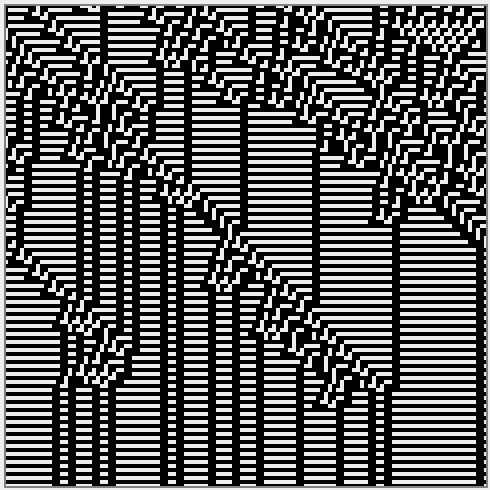
\includegraphics[width=0.8\linewidth]{figures/non_converging_radius2.png}
\caption{Waterfall plot of a radius 2 rule that fails to converge within 300 iterations. The top row is the initial condition, and each successive row is the 
result applying the rule to the row above it.}
\label{fig:waterfall_1}
\end{center}
\end{figure}

\begin{figure}
\begin{center}
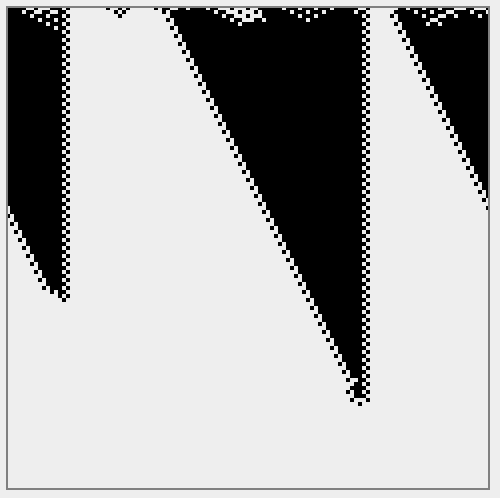
\includegraphics[width=0.8\linewidth]{figures/converging_radius2.png}
\caption{Waterfall plot of a radius 2 rule that successfully classifies an initial condition.}
\label{fig:waterfall_2}
\end{center}
\end{figure}

Figures~\ref{fig:r2_rho} and \ref{fig:r3_rho} plot the performance of an elite $r = 2$ and an elite $r = 3$ rule, respectively, as evolved after 50 generations. As can be seen, performance did not differ significantly; or maybe it did. We'll find out, and put a summary regarding which rule performs better here.

\begin{figure}
\begin{center}
\includegraphics[width=\linewidth]{figures/lambda_correctness_1_r2.eps}
\caption{Performance of two elite, $r = 2$ rules as a function of $\rho$. Each rules' performance was recorded for 1000 ICs with $\rho$ 
varying in intervals of 0.025, and precent correct is plotted. As expected, both rules perform well for extreme values of $\rho$, but 
performance drops as $\rho$ approaches the difficult cases around $\frac{1}{2}$.}
\label{fig:r2_rho}
\end{center}
\end{figure}
\begin{figure} [ht]
\begin{center}

\includegraphics[width=\linewidth]{foo.png}
\caption{Performance of an elite, $r = 3$ rule as a function of $\rho$. As in the case of an elite $r = 2$ rule (fig.~\ref{fig:r2_rho}), the rule performs well when the proportion of \texttt{1}s is 
low or high, but performance drops as $\rho$ approaches the difficult cases around $\frac{1}{2}$.}
\label{fig:r3_rho}
\end{center}
\end{figure}

It is also interesting to compare the performance of the most fit $r = 2$ and $r = 3$ rules over multiple generations. Figures~\ref{fig:r2_best_fit} and 
\ref{fig:r3_best_fit} show the best fitness for a sample run for the two neighborhoods as a function of generation. As can be seen in those figures, both trajectories exhibit `epochs' as described by Mitchell \cite{Mitchell:1994:ECA:186092.186116}: There is an initial plateau interrupted by a jagged rise in 
best fitness, where these increases represent the discovery of new, dominant strategies.

\begin{figure}
\begin{center}
\includegraphics[width=\linewidth]{figures/max_epoch_radius2.eps}
\caption{Best fitness for an $r = 2$ run by generation. The maximum fitness trajectory exhibits epochs: the population rapidly leaves epoch 1, flattens out until about generation 30, and then climbs again to another plateau.}
\label{fig:r2_best_fit}
\end{center}
\end{figure}
\begin{figure} 
\begin{center}
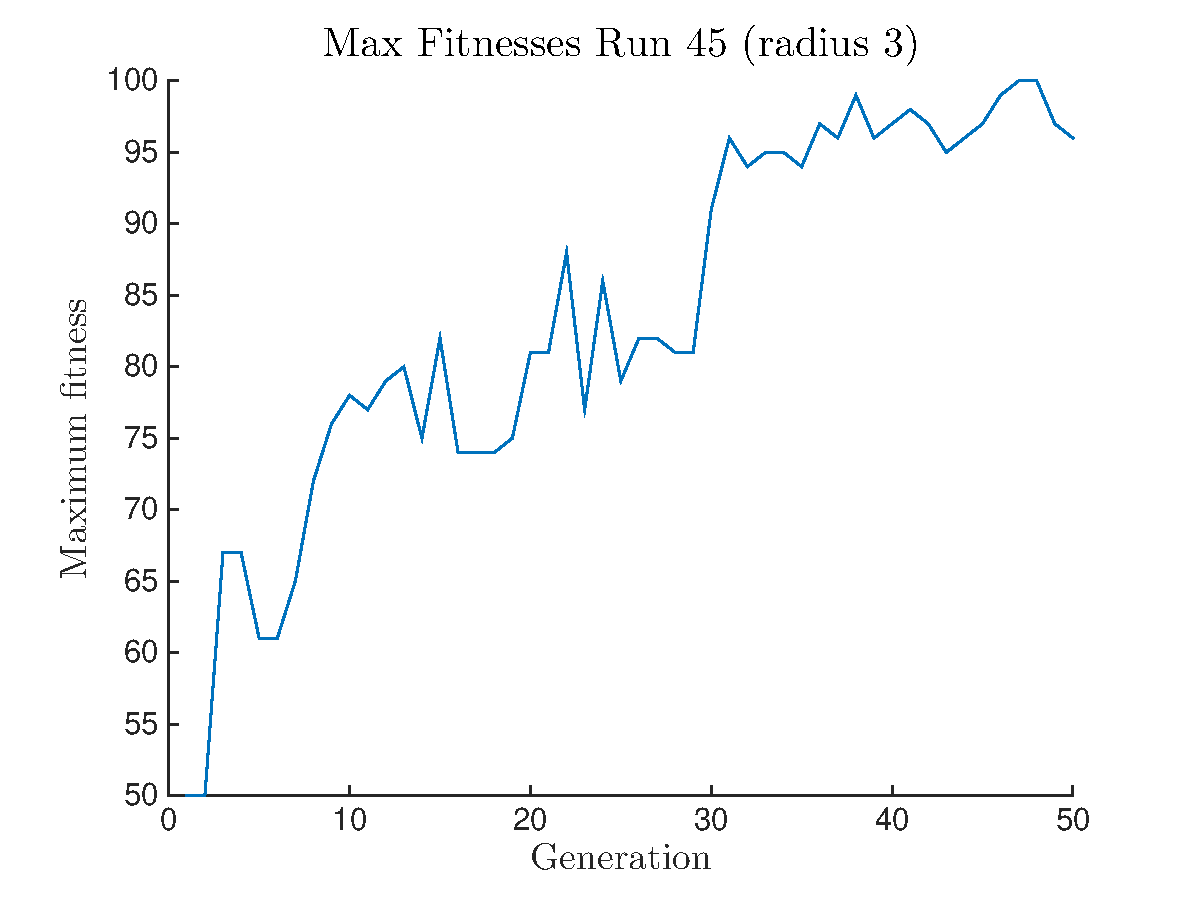
\includegraphics[width=\linewidth]{figures/max_epoch_radius3.eps}
\caption{Best fitness for an $r = 3$ run by generation. As in the case of $r = 2$ (fig.~\ref{fig:r2_best_fit}), the trajectory exhibits epochs; in this case, there appear to be three plateaus.}
\label{fig:r3_best_fit}
\end{center}
\end{figure}

Let $\lambda$ be the proportion of \texttt{1}s in the binary representation of a rule (section~\ref{sec:methods}). Then the transitions just described are 
equivalent to shifting from rules with $\lambda = 0$ or $\lambda = 1$ to rules with $\lambda \approx \frac{1}{2}$. This transition is depicted in 
figures~\ref{fig:histogram_r2} and~\ref{fig:histogram_r3}, for $r = 2$ and $r = 3$ runs, respectively.

\afterpage{%
\begin{figure*}
\begin{center}
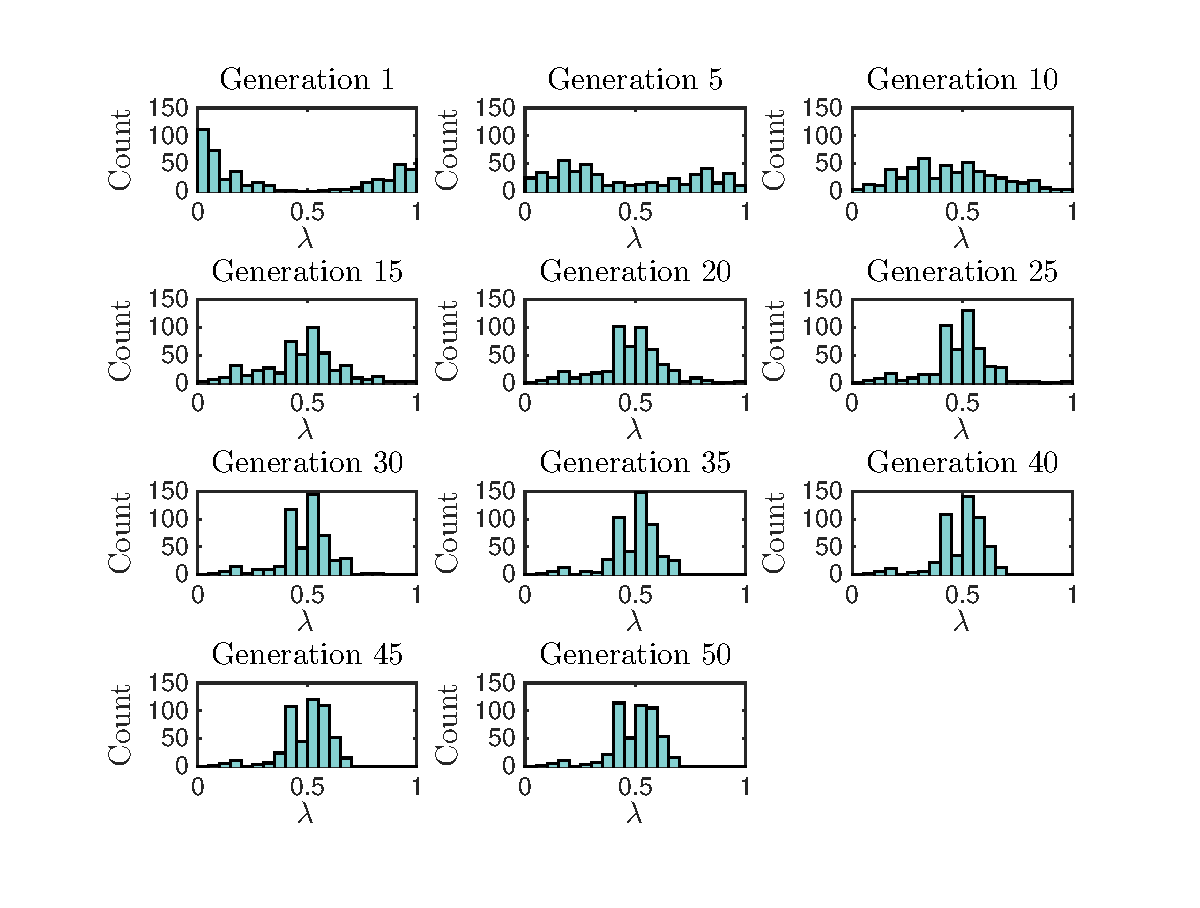
\includegraphics[width=\textwidth]{figures/histograms_r2.eps}
\caption{Frequency of different elite rules (as represented by $\lambda$) by generation, for 50 $r = 2$ runs. Generations 1 and 2 are biased towards $\lambda \approx 1.0$ and $\lambda \approx 0.0$ indicating that successful rules converged on all \texttt{0}s or all \texttt{1}s, regardless of $\rho_0$. By generation 15 
successful rules are starting to cluster near $\lambda = 0.5$, and we can also see the characteristic 'dual peaks' resulting from counting both rules that 
began life near $\lambda = 0.0$ and those that began near $\lambda = 1.0$.}
\label{fig:histogram_r2}
\end{center}
\end{figure*}
\clearpage
}

\afterpage{%
\begin{figure*}
\begin{center}
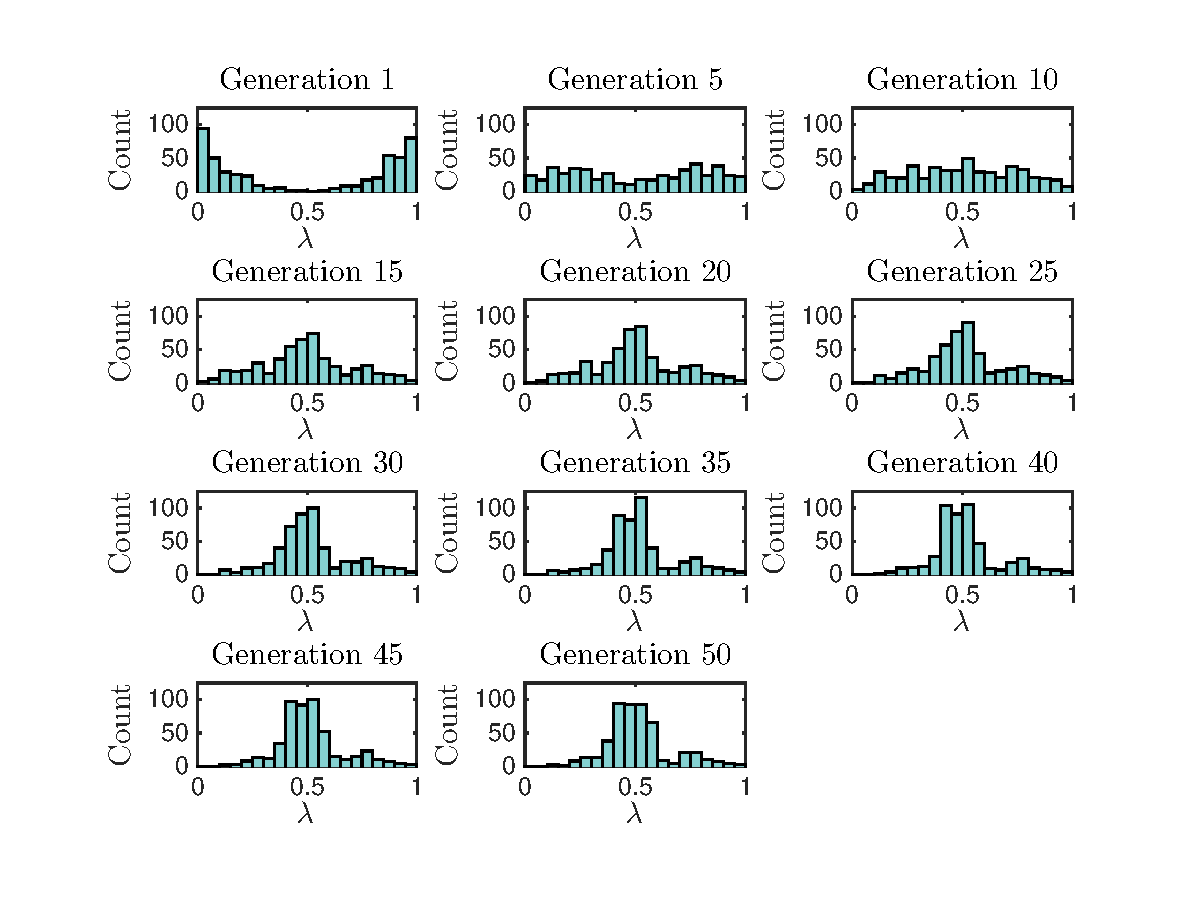
\includegraphics[width=\textwidth]{figures/histograms_r3.eps}
\caption{Frequency of different elite rules (as represented by $\lambda$) by generation, for 50 $r = 3$ runs. Generations 1 and 2 are biased towards $\lambda \approx 1.0$ and $\lambda \approx 0.0$ indicating that successful rules converged on all \texttt{0}s or all \texttt{1}s, regardless of $\rho_0$. By generation 15 
successful rules are starting to cluster near $\lambda = 0.5$, a trend that continues to the final generation.}
\label{fig:histogram_r3}
\end{center}
\end{figure*}
\clearpage
}

Finally, note that each location in the lattice has a transient period in which its state may continue to flip before finally stabilizing (if at all; see figures~\ref{fig:waterfall_1} and \ref{fig:waterfall_2}). One way to quantify this period is to count the number of times a given location changes state 
over the 300 iterations of a rule, given an initial condition. In order to visualize the relation between the length of a transient period and the fitness of a rule, 
we recorded the average length of the transients for each rule on each IC in the test set after each generation, and plotted this value against the fitness 
for that rule (figure~\ref{fig:transients}).

\begin{figure}
\begin{center}

\includegraphics[width=\linewidth]{foo.png}
\caption{Average length of transients for each rule plotted against the fitness of that rule.}
\label{fig:transients}
\end{center}
\end{figure}

\subsection{Mutational robustness} \label{sec:2_2}

Mutational robustness occurs when changes in the genotype are phenotypically neutral: The genomic modification results in no significant change 
in the traits expressed, and hence no difference in fitness \cite{wagner_role_2012}. When a phenotype is robust in this way, it may be possible for the 
genome to move to a very different region of search space by accruing changes over multiple generations, increasing the breadth of the search without 
having to cross low-fitness boundaries.

If our CAs are mutationally robust, then the nearby neighbors of elite rules should themselves perform well. To assess whether 
this is the case, we selected XXXX elite rules from both the $r = 2$ and $r = 3$ runs, and randomly mutated each \textit{x} times, for $x = 1,2,3, ... 7$. 
For each \textit{x}, we tested the resulting rules against a set of ICs and recorded the fitness. The results are given in figure~\ref{fig:robustness}.

\begin{figure}
\begin{center}

\includegraphics[width=\linewidth]{foo.png}
\caption{Testing for the mutational robustness of elite rules. XXXX elite rules from $r = 2$ and $r = 3$ GA runs were chosen and randomly mutated 1, 2, ... 7 
times. After each mutation, the resulting rules were tested against the same set of ICs, and the fitness recorded. As can be seen in the figure, 
rules are robust for approximately YYYY mutations, at which point fitness declines.}
\label{fig:robustness}
\end{center}
\end{figure}

\subsection{In search of a better CA} \label{sec:2_3}

As noted above (figure~\ref{fig:histogram}), some of the earliest successful strategies to emerge are those that (i) go to all \texttt{1}s or all \texttt{0}s by default, 
yet (ii) change their behavior for values of $\rho$ at the opposite extreme. For example, a rule may for the most part map every 
neighborhood to \texttt{0}, except for neighborhoods with many \texttt{1}s, so an IC with a high enough value of $\rho$ will 
`overwhelm' the default behavior of the rule. In such a rule, every IC with $\rho < 0.5$ is successfully classified, as are ICs with $\rho \approx 1.0$, but 
errors are made on those with $\rho \gtrapprox 0.5$.

Of course, the region around $\rho = 0.5$ is precisely the region we want to encourage the rules to deal with, yet under the fitness testing regime 
used for the experiments reported above, the `easy' cases (where $\rho \approx 1.0$ or $\rho \approx 0.0$) appear in testing sets  
with the same probability as any other IC for the entire GA run. As a result, CAs are still being rewarded for dealing with these easy cases long after their 
utility is exhausted.

To address this issue, we modified the GA so that the fitness gain for successfully classifying ICs is a function of its distance from $\rho = 0.5$: The 
closer to 0.5, the more a correct classification is worth. Furthermore, this function is adjusted depending on the current generation, so that at generation 1 
all ICs are worth the same amount of fitness regardless of their distance from $\rho = 0.5$, and the distance becomes increasingly more important as 
the generations progress.

To address this issue, we modified the GA so that IC sets are initially randomly constructed using a uniform distribution, but 
the distribution becomes increasingly normal, with mean of $\rho = 0.5$. This means that as the GA progresses, it becomes less likely that a 
set of ICs will include the easier cases, and more likely that harder cases will be included. 


